\documentclass[a4paper]{article}

\usepackage{INTERSPEECH2015}

\usepackage{graphicx}
\usepackage{amssymb,amsmath,bm}
\usepackage{textcomp}

\def\vec#1{\ensuremath{\bm{{#1}}}}
\def\mat#1{\vec{#1}}


\sloppy % better line breaks
\ninept

\title{Speaker Normalization of DNN-based  Acoustic Models using Partitioned Hidden Layers}

%%%%%%%%%%%%%%%%%%%%%%%%%%%%%%%%%%%%%%%%%%%%%%%%%%%%%%%%%%%%%%%%%%%%%%%%%%
%% If multiple authors, uncomment and edit the lines shown below.       %%
%% Note that each line must be emphasized {\em } by itself.             %%
%% (by Stephen Martucci, author of spconf.sty).                         %%
%%%%%%%%%%%%%%%%%%%%%%%%%%%%%%%%%%%%%%%%%%%%%%%%%%%%%%%%%%%%%%%%%%%%%%%%%%
%\makeatletter
%\def\name#1{\gdef\@name{#1\\}}
%\makeatother
%\name{{\em Firstname1 Lastname1, Firstname2 Lastname2, Firstname3 Lastname3,}\\
%      {\em Firstname4 Lastname4, Firstname5 Lastname5, Firstname6 Lastname6,
%      Firstname7 Lastname7}}
%%%%%%%%%%%%%%% End of required multiple authors changes %%%%%%%%%%%%%%%%%

\makeatletter
\def\name#1{\gdef\@name{#1\\}}
\makeatother \name{{\em Lahiru Samarakoon, Khe Chai Sim}}

\address{School of Computing, National University of Singapore, Singapore \\
  {\small \tt lahiruts@comp.nus.edu.sg, simkc@comp.nus.edu.sg}
}

%\twoauthors{Karen Sp\"{a}rck Jones.}{Department of Speech and Hearing \\
%  Brittania University, Ambridge, Voiceland \\
%  {\small \tt Karen@sh.brittania.edu} }
%  {Rose Tyler}{Department of Linguistics \\
%  University of Speechcity, Speechland \\
%  {\small \tt RTyler@ling.speech.edu} }

%
\begin{document}

  \maketitle
  %
  \begin{abstract}
    This paper proposes a modified feed-forward DNN structure for acoustic modeling that is trained progressively in a speaker-aware fashion using i-vectors.  The concept of Partitioned Hidden Layer  is introduced.  In partitioned hidden layers, a separate set of  hidden nodes are allocated to transform speaker information. The idea is to learn a global transformation for speaker features to implicitly minimize the mismatch due to the inter-speaker variability. Experiments on the TIMIT phone recognition task show  4.7\% relative improvement when compared with a strong baseline trained on speaker adapted features.  Furthermore, the proposed approach reported significantly better results compared to the standard i-vector based method. We also report a detailed comparison of our approach with similar speaker-aware training approaches that employ i-vectors. 
    
  \end{abstract}
  \noindent{\bf Index Terms}: Automated speech recognition, deep neural networks, implicit speaker normalization.


  \section{Introduction}

    Recently, Deep Neural Network (DNN) based acoustic modeling has achieved state-of-the-art performance in Automatic Speech Recognition (ASR) systems  in comparison to the conventional Gaussian Mixture Model (GMM) based systems \cite{Hintonatel}. The increased computational power and the utilization of the Graphical Processing Units (GPUs) in computations have made the training of these complex models affordable. Moreover, the advances in machine learning approaches in DNN training have also contributed to the increased performance. DNN-HMM systems surpass the conventional GMM-HMM systems by using the superior representation learning power of the DNNs to model senone log-likelihood, combined with the sequential modeling capability of HMMs to model speech signals. 
    
    
    DNNs, like all other machine learning techniques, are susceptible to performance degradation due to the mismatch between the training and testing conditions. Adaptation techniques change the model to match the testing condition or change the inputs to match the model. In ASR, speaker adaptation techniques are used to optimize the performance by minimizing the training-testing mismatch introduced by the speaker variability. The two most successful ways of adapting a GMM-HMM model is to use the maximum a posteriori (MAP) \cite{MAP} and maximum likelihood linear regression (MLLR) \cite{MLLR} techniques. In MAP, instead of using maximum likelihood for  parameter estimation, model parameters are re-estimated by maximizing the posterior probability.  In MLLR, a linear transformation of the model parameters are estimated to construct the adapted model. It is possible to take advantage of GMM-HMM adaptation techniques with tandem systems \cite{Tandem}\cite{Tandem2} in which a DNN is trained to extract bottleneck features for a GMM-HMM system. 
    
    The adaptation techniques developed for generative GMMs cannot be directly utilized for discriminative DNNs. In addition, due to the large number of parameters in DNN-HMM systems, techniques developed for ANN-HMM hybrid systems \cite{ANN} are prone to over-fitting when only a small amount of adaptation data is available. However, DNN adaptation is important as it reduces the error rates significantly \cite{KLDNN}\cite{IVECT}\cite{IVECT1}\cite{SPEAKECODE1}.  A good adaptation technique should prevent over-fitting to the adaptation data. This is achieved by finding a compact representation of the model parameters or using a regularization based method to perform the adaptation conservatively.  Moreover, it is desirable to perform adaptation in an unsupervised fashion, which is more realistic.
  
    
    In this paper, we propose a modified DNN structure which is speaker adaptively trained on acoustic features concatenated with the i-vectors \cite{IVECT2}\cite{IVECT3}. The i-vectors can be considered as low dimensional representations of the speaker characteristics. The concept of Partitioned Hidden Layers is introduced which has a separate partition of hidden units to learn a better speaker representation. This facilitates the learning of a global transformation for the i-vectors.  DNN is capable of using this extra information about the speakers to perform implicit speaker normalization.
    
    
    The rest of the paper is organized as follows. In Section 2, a brief review of the DNN adaptation techniques are given. Section 3 describes our approach based on partitioned hidden layers. Experimental results are reported in Section 4 and we conclude our work in Section 5. 

  
 
 \section{DNN Adaptation}
 

 DNN adaptation techniques can be categorized into three classes: linear transforms, regularization methods, and subspace methods.
 
 Linear Transformation based methods augment the original DNN model with a linear layer. Usually, the linear layer is initialized with an identity matrix and zero biases and are updated with the back-propagation (BP) algorithm using the adaptation data while keeping the weights of the original DNN fixed. In linear input network (LIN) \cite{LIN1}\cite{LIBO} and feature discriminative linear regression (fDLR) \cite{FDLR}, a linear layer is inserted above the input layer and the first hidden layer. The intuition is similar to fMLLR \cite{MLLR} where speaker dependent (SD) features are linearly transformed to match the speaker independent (SI) model. When the linear transformation is applied to the softmax layer the adaptation technique is known as linear output network (LON) \cite{LIBO}. The intuition is to transform the last hidden layer's SD feature representation to match the average speaker. Depending on the number of output neurons, it is possible to apply the transformation before or after the softmax layer weights. When the linear transformations is applied to the hidden layers, it is known as the linear hidden network (LHN) \cite{LHN}. 
 
 The adaptation of all the parameters is more powerful, hence more effective than the linear transformations. However, this may lead to over-fitting since the amount of adaptation data is limited. Conservative training methods address this issue by adding a regularization term to the adaptation criterion. In \cite{KLDNN}, a KL divergence based method is used to force the distribution of the adapted model to be closer to that of the SI model. The estimated distribution is a linear interpolation between the target distribution (derived using alignments) and the distribution of the SI model. Another popular approach is the $L_2$ regularization \cite{L2}, which aims to keep the parameters of the adapted model closer to that of the SI model. However, speaker personalization of all the parameters increases storage costs, which necessitates the employment of techniques that reduce per-speaker footprint \cite{FOOTPRINT}.  Therefore, some approaches perform the adaptation on a subset of parameters, including the last hidden layer \cite{RLL}, output layer biases \cite{OUTBIASES}, or more active hidden units of the network \cite{RLL}. 
 
 
 It is also possible to find a speaker subspace and perform the adaptation as a point in the subspace. In \cite{PCA}, principal component analysis (PCA) is performed on a set of adaptation matrices to get eigenvectors. Then, transformations for test speakers can be estimated as a linear combination of these eigenvectors. Coefficients for each speaker is estimated using the BP procedure. This method can also be used with the LIN, LHN and LON techniques \cite{LIBO}.  Another popular subspace method is to feed the features for speaker variability with acoustic features. These methods are discussed in Section 3 along with comparisons to the techniques we propose in this paper.
 
 
 \section{Proposed Method}
 
   A DNN can be viewed as a model that learns a feature representation as well as a classifier. Each hidden layer learns a more abstract representation ($\mathbf{h}^l$) from the lower layer's representation ($\mathbf{h}^{l-1}$), which can be shown as:
  
  \begin{equation}
  \label{standard}
  \mathbf{h}^l = \sigma (\mathbf{W}^l \mathbf{h}^{l-1}+ \mathbf{b}^l )
  \end{equation} where $\sigma$ is the sigmoid activation function. $\mathbf{W}^l$ and $\mathbf{b}^l$ are the weight matrix and the bias vector for layer $l$, respectively. 
  
   
   In the proposed method, we incorporate speaker information in addition to the standard acoustic features during training. This approach is known as speaker-aware training. 
  
   \subsection{Speaker-aware Training (SaT)}
   
  The intuition behind SaT is that a DNN is capable of exploiting the supplementary information about speakers to adjust the model parameters for speaker normalization. The first step in SaT is the speaker information estimation where techniques like i-vectors \cite{IVECT}\cite{IVECT1}\cite{IVECT4} and bottleneck features \cite{HENGUAN} are commonly used. In this paper, i-vectors are used as the speaker information. However, it is also possible to replace the i-vectors with the bottleneck features. 
  
   \begin{figure}[ht]
     	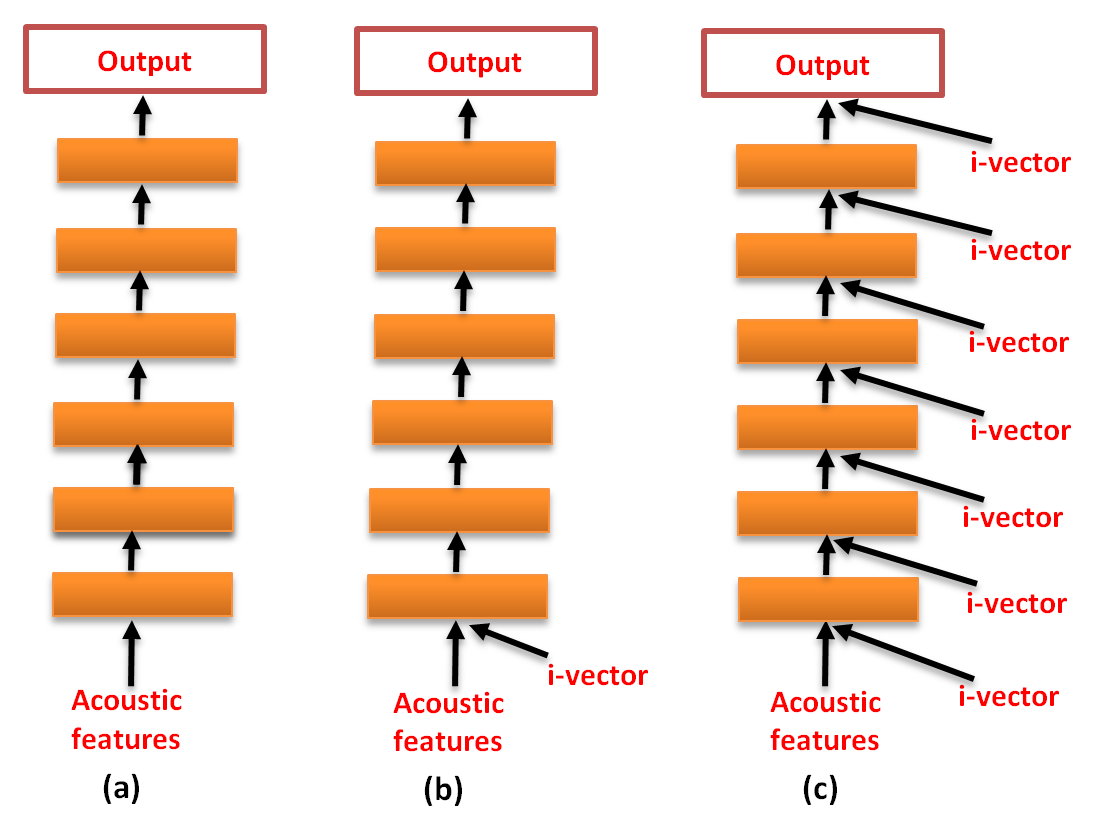
\includegraphics[width=\linewidth]{figure4.png}
     	\caption{Illustration of different DNN model structures. a) Standard System b) i-vector System c) Extended i-vector System}
     	\label{fig:diagram1}
     \end{figure}
     
    The simplest approach in SaT is to concatenate the acoustic features with the i-vector of the speakers before DNN training.  Figure \ref{fig:diagram1}(b) shows the resulting structure of the network, which is referred as the \emph{i-vector baseline} throughout this paper (Figure \ref{fig:diagram1}(a) shows a DNN when only the acoustic features are used.) \cite{IVECT}\cite{IVECT1}\cite{IVECT4}. Furthermore, hidden layer representations are considered as more abstract representations of the DNN inputs. Therefore, it is also possible to concatenate hidden layer representations with the appropriate i-vector. The resulting model when the DNN inputs and hidden layer representations at all levels are concatenated with i-vectors is shown in Figure \ref{fig:diagram1}(c). We refer to this model as the \emph{Extended i-Vector System}. The extended i-vector system is similar to the so-called speaker code \cite{SPEAKECODE1} approach. However, in speaker code, speaker information is estimated during training, whereas the i-vector estimation is independent from DNN training. 
      
    As shown below,  speaker information can be considered as a bias when the input signal for that layer is augmented with it.
  
   \begin{equation}
   \label{sat1}
   \mathbf{h}^l = \sigma (\mathbf{W}^l \mathbf{h}^{l-1}+ \mathbf{b}_s^l )
   \end{equation} where $\mathbf{b}_s^l$, the speaker dependent bias for layer $l$, is given by
   
   
   \begin{equation}
   \label{sat2}
   \mathbf{b}_s^l =  \mathbf{W}_s^l \mathbf{s}^l + \mathbf{b}^l 
    \end{equation}   $\mathbf{s}^l$ is the speaker representation and  $\mathbf{W}_s^l$ is the speaker representation transformation weight matrix for layer $l$, respectively. 
    
     
   In all the models shown in Figure \ref{fig:diagram1}, the i-vectors are connected to the hidden layers directly.  However, some works have shown gains from learning i-vector representations  using non-linear transformations \cite{IVECDNN}.  This has prompted us to add a set of hidden units to non-linearly transform the i-vectors as shown in Figure \ref{fig:diagram2} (b) before connecting the i-vectors to the standard network.   When one layer of hidden units are used to transform i-vectors, the speaker dependent bias $\mathbf{b}_s^l $ is given by:
   
    \begin{equation}
    \label{sat3}
    \mathbf{b}_s^l =  \mathbf{W}_{s1}  \sigma ( \mathbf{W}_{s0}^l \mathbf{s}^l + \mathbf{b}_{s0}^l )  +   \mathbf{b}^l 
    \end{equation}  where $\mathbf{W}_{s0}$,$\mathbf{W}_{s1}$ are  weight matrices and $\mathbf{b}_{s0}^l $ is the bias vector for the transformation.
   
   It is also possible to add more than one layer of speaker representative hidden units. In this paper, two such systems are trained. The first system applies the non-linear transformation to i-vectors using a layer of  speaker representative hidden units whereas in the second system two such layers are used. In the case of two layers of i-vector transformations, the speaker dependent bias $\mathbf{b}_s^l$ is given by
   
    \begin{equation}
    \label{sat4}
    \mathbf{b}_s^l =  \mathbf{W}_{s2}  \sigma(\mathbf{W}_{s1}  \sigma ( \mathbf{W}_{s0}^l \mathbf{s}^l + \mathbf{b}_{s0}^l  ) + \mathbf{b}_{s1}^l ) +   \mathbf{b}^l 
    \end{equation}  where $\mathbf{W}_{s0}$,$\mathbf{W}_{s1}$ , $\mathbf{W}_{s2}$ are weight matrices and $\mathbf{b}_{s0}^l$,$\mathbf{b}_{s1}^l$ are bias vectors for the transformation. 
   
    Intuitively, these transformations of the i-vectors should help, as it provides more capacity to learn a suitable abstraction of the speaker information.      

 \begin{figure}[ht]
 	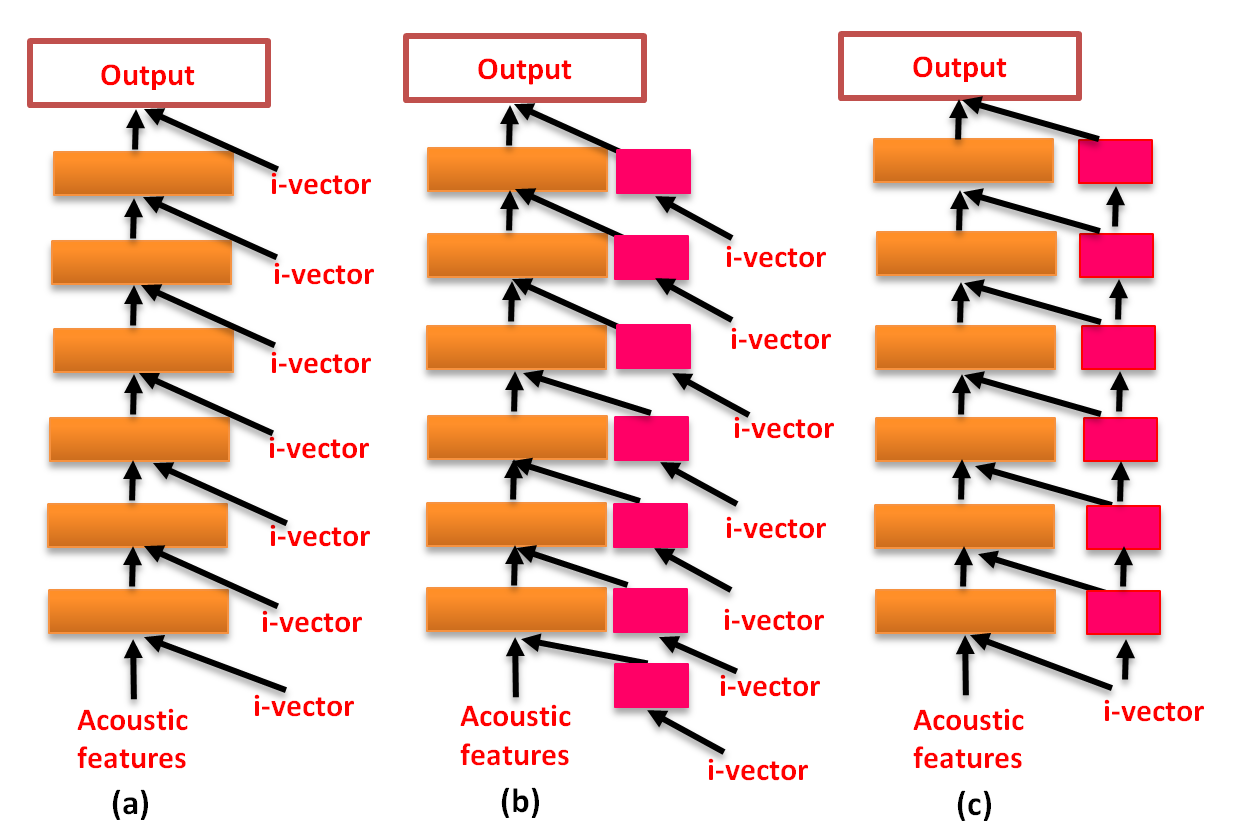
\includegraphics[width=\linewidth]{figure3.png}
 	%\includegraphics[height=4in, width=2.2in]{prgressLearning.png}
 	\caption{(a) Extended i-vector system  (b) Extended i-vector system with non-linear transformations  (c) Partitioned DNN }
 	\label{fig:diagram2}
 \end{figure}
 
 \subsection{Partitioned Hidden Layers}
 
 The addition of the non-linear transforms to the extended i-vector systems increases the model complexity. Furthermore, this also raises the design question of the number of necessary transformation layers.  Therefore, we propose to include a speaker representation transformation to the hidden layers of the DNN.  
 
 The proposed approach adapts a partitioned hidden layer (PHL) architecture, which has two partitions of hidden units. The first partition is known as the standard partition, which learns the acoustic feature representations ($\mathbf{h}^l$), and the second (speaker) partition  is to learn the speaker representations ($\mathbf{s}^l$). The standard partition of the hidden layer receives signals from both partitions of the lower layer, whereas the speaker partition of the hidden layer receives the input signal only from the speaker partition of the lower layer.  PHL $l$  can be represented as below.
 
 \begin{equation}
 \label{partitioned_standard}
 \mathbf{h}^l = \sigma (\mathbf{W}^l \mathbf{h}^{l-1}+ (\mathbf{W}_s^l \mathbf{s}^{l-1} + \mathbf{b}_{h}^l ))
 \end{equation}
 \begin{equation}
 \label{partitioned_speaker}
 \mathbf{s}^l = \sigma (\mathbf{W}_t^l \mathbf{s}^{l-1}+ \mathbf{b}_{t}^l )
 \end{equation} where $\mathbf{W}^l$ and   $\mathbf{W}_s^l$ are the weights matrices for the acoustic and speaker features that are connected to the standard hidden units and $\mathbf{b}_{h}^l$ is the bias vector. $\mathbf{W}_t^l$ and $\mathbf{b}_{t}^l$ are the weight matrix and bias vector associated with speaker information transformation respectively. The resulting model when all the hidden layers of the network are PHLs is given in Figure \ref{fig:diagram2} (c) and we refer to this model as the \emph{Partitioned DNN}.

\subsection{Training configuration}

 All the models with speaker features are trained using a warm-start configuration to reduce the training time. In warm start,  the weights of the initial DNN is directly used and the weights for the additional connections are randomly initialized. Then, the fine-tuning of the model is done in two steps. First, the newly added random weights are fine-tuned while keeping the rest of the weights fixed to ensure that the new weights contribute towards the learning objective. In the second step, all the weights are fine-tuned together.  
 
 Furthermore, the training of the SaT DNNs is carried out progressively. For instance, the Partitioned DNN is trained as follows.  Starting from the initial DNN, we first trained the i-vector  baseline using the warm-start configuration as described above.  Then the first hidden layer is replaced with a PHL and trained until convergence. Next,  the second hidden layer is replaced with a PHL and trained.  Likewise, this procedure is continued until all the hidden layers of the network are PHLs.  Similarly, all the extended i-vector systems are trained progressively. The progressive learning from the bottom to top facilitates the investigation of  the  performances of the intermediate models as well as the final model. 

 \section{Experiments}
 
 \subsection{Experimental Setup}
 
 In this paper, all the experiments are performed on the TIMIT corpus. The standard training set of 462 speakers is used with all the SA sentences removed. A development set of 50 speakers are used in meta parameter tuning. We report the results on the standard core test set of 24 speakers. 
 
First, MFCC features are extracted from speech using 25ms window and a 10ms frame-shift. Then, cepstral mean normalization (CMN) per speaker is applied to the MFCCs. Linear discriminant analysis (LDA) features are obtained by first splicing 7 frames of 13-dimensional MFCCs and then projecting down to a 40 dimension using LDA.  A global semi-tied covariance (STC) transformation \cite{STC} is applied on top of the LDA features.  The final set of speaker adapted features are obtained by applying a speaker specific feature-space maximum likelihood linear regression (fMLLR) transform. The GMM-HMM system for generating the alignments for DNN training is built on top of these 40 dimensional fMLLR features.  


The initial DNN-HMM baseline is also trained on the fMLLR features that span a context of 11 neighboring frames.  Before being presented to the DNN, cepstral mean and variance normalization (CMVN) is performed on the fMLLR features globally.  Generative pre-training is performed using Restricted Boltzmann Machines (RBMs).  The initial DNN has  6 sigmoid hidden layers with 1024 units per layer, and 2042 senones as the outputs.  All the DNNs are trained to optimize the cross-entropy criterion with a mini-batch size of 256.  We used the Newbob learning rate schedule with an initial learning rate of 0.008.  Kaldi toolkit \cite{KALDI}  is used for GMM-HMM system building and in training of the initial DNN baseline.  We employed the Theano framework \cite{Theano2} to train i-vector systems and the Partitioned DNN with warm start and progressive learning. 

The i-vectors are trained on top of the same 40 dimensional fMLLR features. The UBM consist of 128 gaussians. We extracted i-vectors that are of 25 dimension.  Kaldi's in-built i-vector tools are used in extracting i-vectors \cite{KALDI}. 

 
 \subsection{Results}
 
 \begin{table}[t]
 	\renewcommand{\arraystretch}{1.3}
 	\caption{PER (\%) of various DNN models on test and dev sets. Relative improvement over the baseline is given in brackets. }
 	\label{tbl:results}
 	\centering
 	\begin{tabular}{|c|c|c|}	
 		\hline
 		Model & test set & dev set  \\
 		\hline
 		\hline
 		Initial DNN & 19.1  & 18.3 \\
 		\hline
 		i-vector baseline & 18.7 (2.1) & 17.8 (2.7) \\
 		\hline
 		Extended i-vector  & 18.7 (2.1)  & 17.6 (3.8)\\
 		\hline
 		Extended i-vector 1-layer & 18.5 (3.1)  & 17.9 (2.7)\\
 		\hline
 		Extended i-vector 2-layer & 18.7 (2.1) & 17.7 (3.3) \\
 		\hline
 		Partitioned DNN & \textbf{18.2} (4.7) & \textbf{17.5} (4.4)\\
 		\hline
 	\end{tabular}		
 \end{table}
 
 
 Table \ref{tbl:results} presents the results for various models for their final configurations. It can be clearly seen that adding speaker information consistently improves the performance over the initial baseline system.  However, these improvements are relatively small. This is simply because the fMLLR features are already transformed to reduce the mismatch due to speaker variability. Both the i-vector (Figure \ref{fig:diagram1}(b)) and the extended i-vector systems (Figure \ref{fig:diagram1}(c))  reported the same result of 18.7\%. The extended i-vector system with two-layer non-linear transformation applied to the i-vectors reported the same performance of 18.7\%.  The extended i-vector system with one-layer non-linear transformation applied to the i-vectors (Figure \ref{fig:diagram2}(b)) improved the performance further to 18.5\%. Partitioned DNN (Figure  \ref{fig:diagram2}(c))  achieves the best performance of 18.2\% which is a 4.7\% relative improvement over the baseline model. It is also worthwhile to mention that only the Partitioned DNN performance is statistically significantly better  than that of the i-vector baseline model.  Since the extended i-vector system with two-layer non-linear transforms has more parameters than the partitioned DNN, the gain of the partitioned DNN is not due to the increased number of parameters. We believe that the gain comes from learning this global transformation of  speaker information. In addition, PHLs facilitates the learning of a similar level of abstract representation for speaker information as the representations in the standard partition. 
 
  \begin{table}[ht]
  	\caption{PER (\%) on the development set as a function of the speaker representation size of PHLs}
  	\label{tbl:dimensions}
  	\begin{center}
  		\begin{tabular}{|c|c|c|c|}	
  			\hline
  			Units & 50 & 100 & 150  \\
  			\hline
  			\hline
  			Partitioned DNN & 17.6 & 17.5 & 17.7 \\
  			\hline
  		\end{tabular}		
  	\end{center}	
  \end{table}
  
 
 
 Table \ref{tbl:dimensions} shows how the PER (\%) changes with the size of the speaker representation in PHLs. The following results are for the final model where all the layers are PHLs. It can be clearly seen that the best performance on the dev set is reported when the dimension is equal to 100. Consequently, in all experiments, 100 is used as the dimensionality of the speaker representation in PHLs. Therefore, PHLs in this paper, have a total of 1124 hidden units with 1024  for the standard partition and 100 for the speaker partition.  Furthermore, we used 100 hidden units to transform the i-vectors in the extended i-vector systems with non-linear transforms. 
 
 
  \begin{figure}[ht]
  	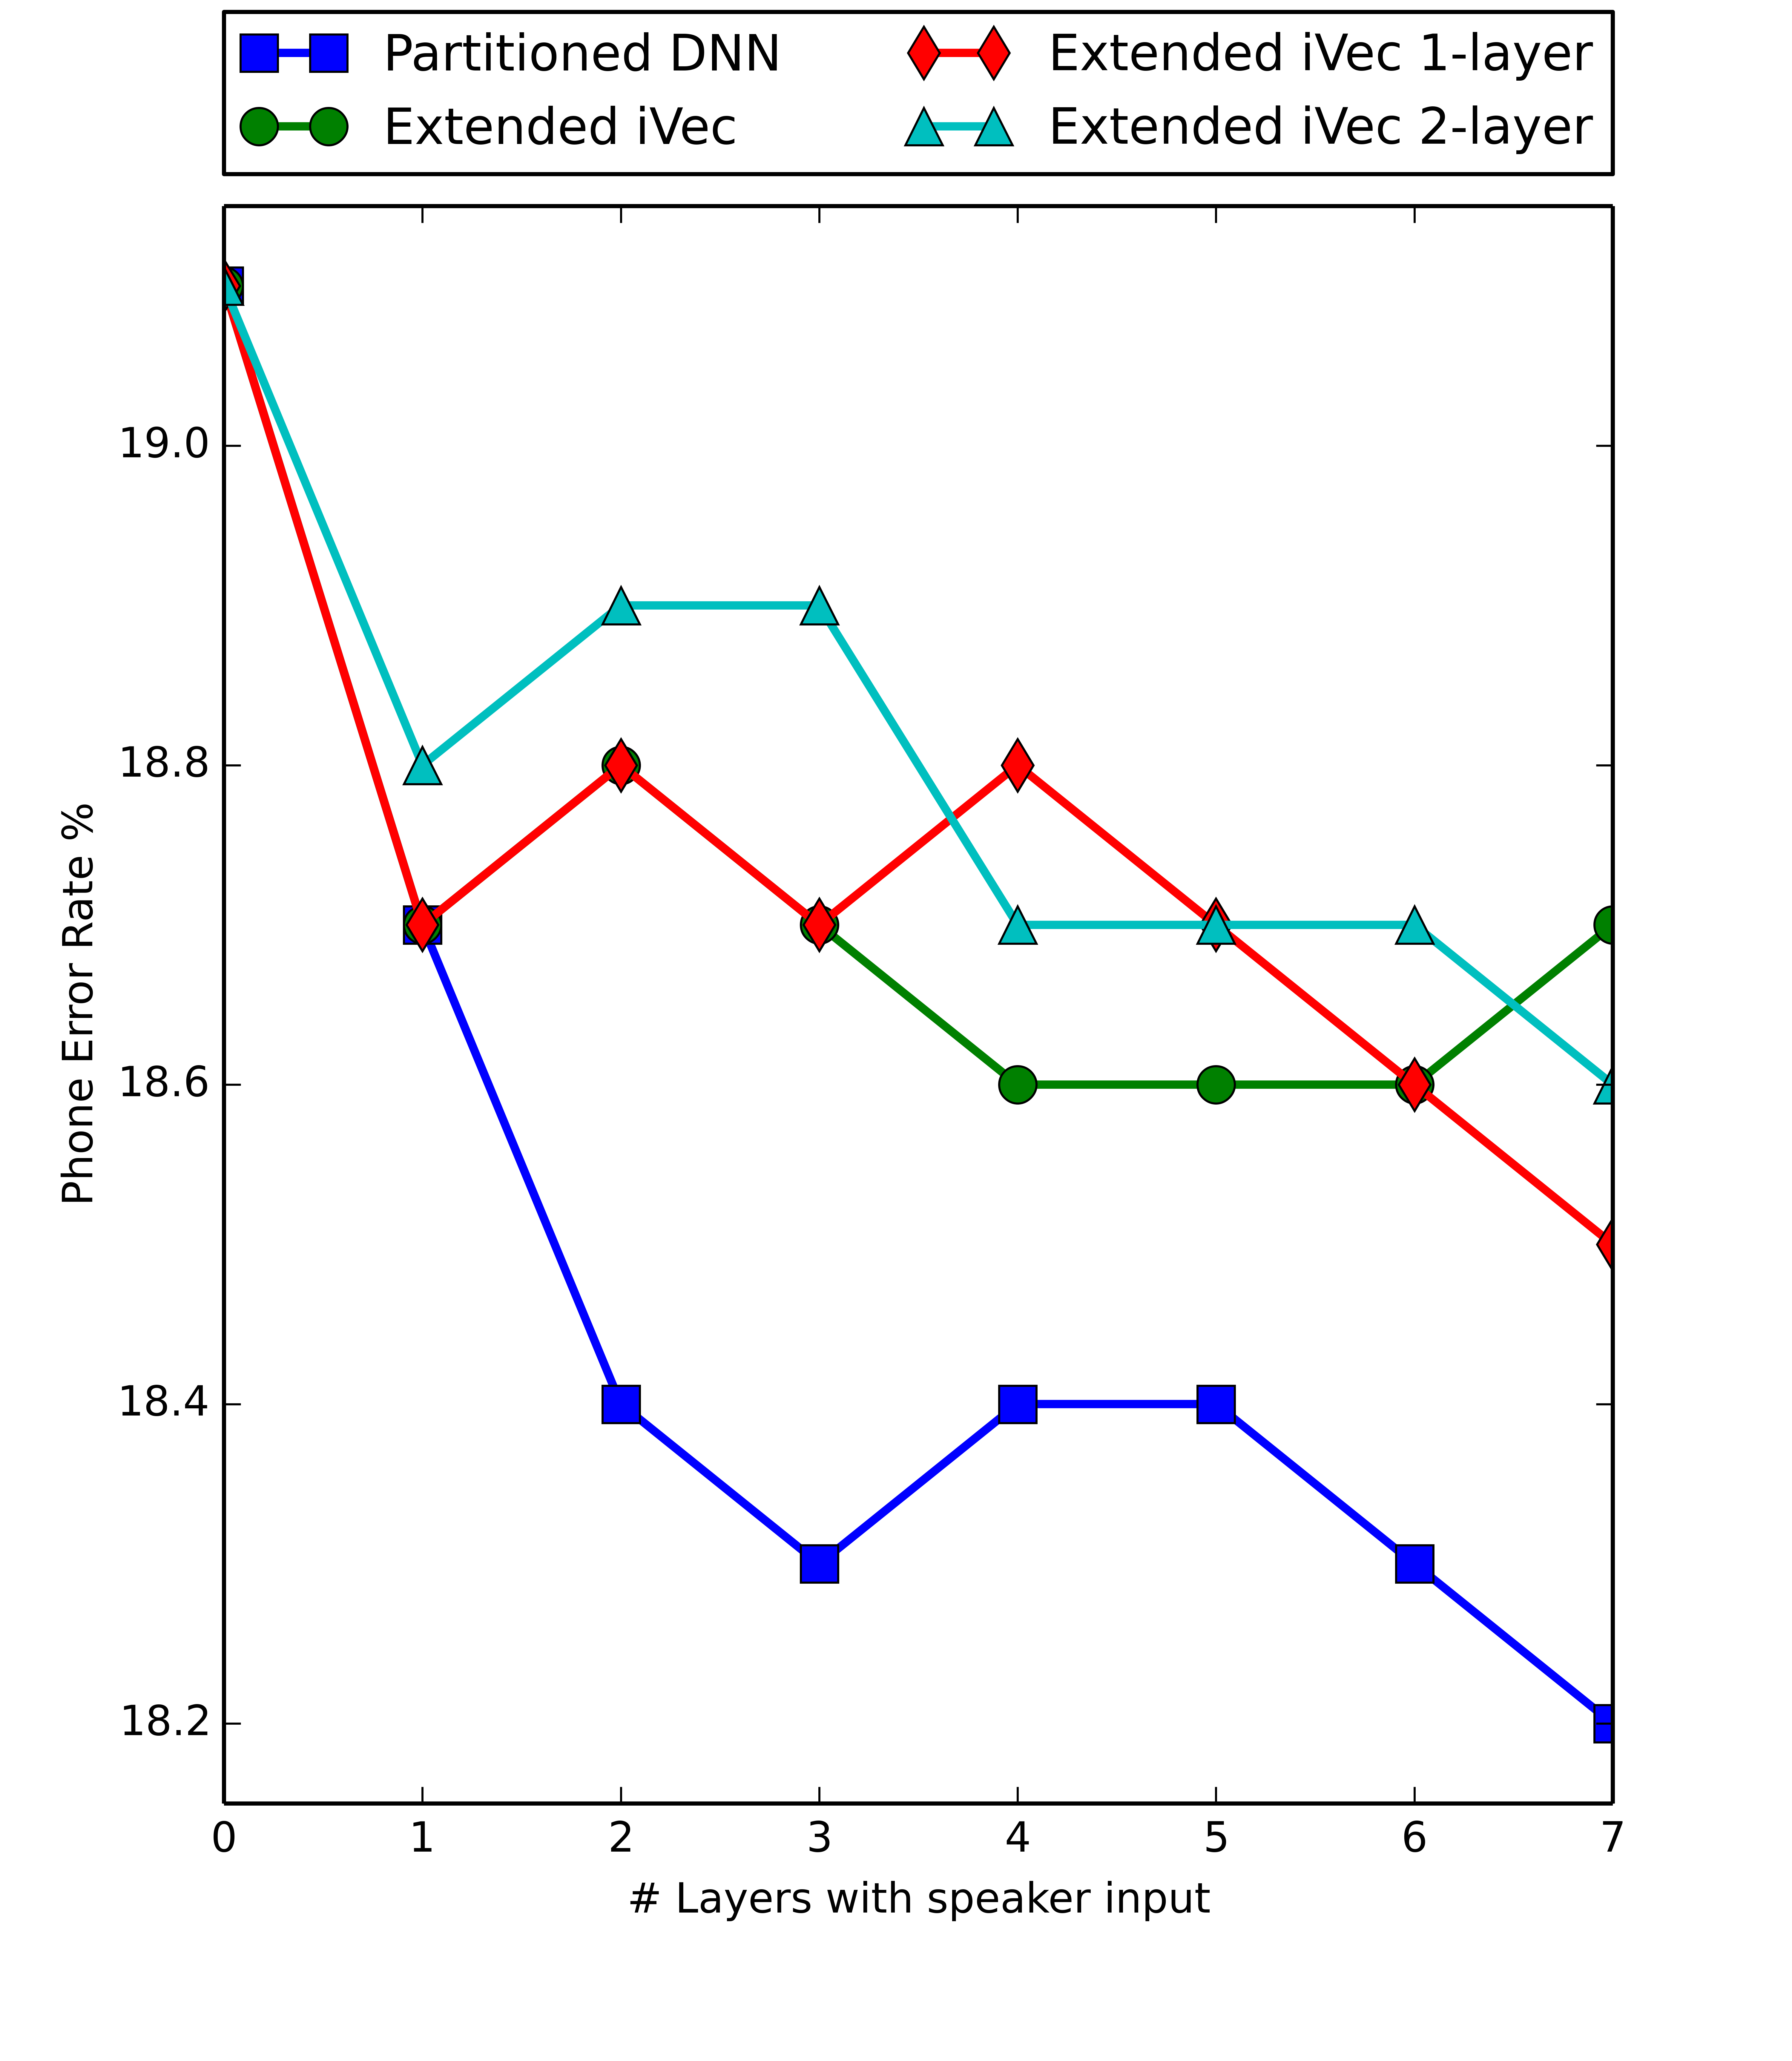
\includegraphics[width=\linewidth]{compare.png}
  	\caption{PER (\%) for various models against the number of layers with speaker input at different stages  during Progressive Learning. Layer 7 is the output layer.}
  	\label{fig:diagram3}
  \end{figure}
  
  Figure \ref{fig:diagram3} shows the PER (\%) for various models at different stages  during progressive learning.  All the models start the progressive learning from the same model, which is the initial DNN baseline. In addition, when the number of speaker layers is one, both partitioned DNN and the extended i-vector system share the i-vector baseline system with an improvement of 0.4\%. When the extended i-vector system with one-layer transform is connected to the first hidden layer, the same improvement is observed in the performance (0.4\%). However,  the extended i-vector system with two-layer transform gives an improvement (0.3\%) which is slightly worse than that of the other models. This can be due to over-fitting when 2 layers are used to estimate the non-linear transformation. Excluding the case where the speaker information is connected to 4 layers, the PER of the partitioned DNN decreased gradually. Furthermore,  all the final models that learn non-linear transformations of the i-vectors report the best performances. 
  
  This also implies that different layers need different levels of transformations of the i-vector for better performance. However, training a system with different levels of non-linear transformations raises lot of design questions and increases the training time. Therefore, partitioned hidden layer approach can be used as a simpler method that can provide different levels of abstractions of the speaker information to the DNN properly. 
  
  Finally, we performed unsupervised adaptation by updating the i-vector for the test speakers. This  reported no improvements. This can be due to the fact that the i-vectors are not updated during training.  As a future work we will update the i-vectors during training to investigate the performance gain for explicit adaptation.  
 
 \section{Conclusions}
 
 In this paper, we have presented a technique that incorporates speaker information to normalize the inter-speaker variability of  the DNN based acoustic models.  Our method relies on the concept of partitioned hidden layer that utilizes two partitions of hidden units. The first partition learns the acoustic feature representations, and the second partition learns the speaker representations. Therefore, by stacking multiple partitioned hidden layers, a global transformation for the speaker representations can be learned which is beneficial for speaker normalization.  Results on the TIMIT phone recognition task show relative improvements of 4.7\% on top of the baseline system trained using the fMLLR features. The performance of this method is also statistically significantly better than that of the standard i-vector based method \cite{IVECT}\cite{IVECT1}\cite{IVECT4}. 
 
  \newpage
  \eightpt
  \bibliographystyle{IEEEtran}

  \bibliography{mybib}

\end{document}
